\subsection{Configuration du stockage}
\subsubsection{Test des disques}
Le test des disques permet de s'assurer de l'intégrité des disques durs avant de les utiliser.
\begin{itemize}
    \item Ouvrir le \textit{Gestionnair de stockage} depuis le menu principal
    \item Accéder à la partie \textit{HDD/SSD}
    \item Cliquer sur le premier disque et ouvrir les \textit{Infos sur la santé}
    \item Accéder à l'onglet \textit{S.M.A.R.T.} et lancer un test étendu
    \item Répéter l'opération pour chaque disque
\end{itemize}

\begin{tip}
Pour certains modèles de disques, des options de contrôle d'intégrité supplémentaires sont disponibles (IronWolf avec les disques Seagate par exemple). Il est recommandé de les activer pour une meilleure fiabilité. Également, les disques de marque Synology peuvent être mis à jour directement depuis DSM.
\end{tip}

La programmation de tests réguliers est recommandée pour s'assurer de la bonne santé des disques.\\
\begin{itemize}
    \item Ouvrir le \textit{Gestionnair de stockage} depuis le menu principal
    \item Accéder à la partie \textit{HDD/SSD}
    \item Ouvrir les \textit{Paramètres}
    \item Depuis le \textit{planificateur de test}, créer une nouvelle tâche de test S.M.A.R.T. quotidienne (test rapide)
    \item Depuis le \textit{planificateur de test}, créer une nouvelle tâche de test S.M.A.R.T. hebdomadaire (test étendu)
\end{itemize}

\begin{tip}
Si d'aures tests sont disponibles, il est recommandé de les activer également.
\end{tip}

\subsubsection{Configuration du volume logique}
Le volume logique correspond au volume de stockage qui sera utilisé pour héberger les machines virtuelles. La configuration est réalisée uniquement depuis le premier NAS, en suivant les étapes suivantes:
\begin{itemize}
    \item Ouvrir le \textit{Gestionnaire de stockage}
    \item Accéder à la partie \textit{Stockage}
    \item Créer un nouveau groupe de stockage
    \item Choisir le type de RAID (dans l'architecture retenue, \textit{Basic}) (figure \ref{fig:03-storage-01})
    \item Sélectionner le(s) disque(s) à utiliser pour le groupe de stockage (figure \ref{fig:03-storage-02})
    \item Créer un volume logique (figure \ref{fig:03-storage-03})
    \item Choisir un système de fichiers (dans l'architecture retenue, \textit{Btrfs}) (figure \ref{fig:03-storage-04})
    \item Valider la création du groupe de stockage, du volume logique et du système de fichiers
\end{itemize}

\begin{important}
Le RAID SHR n'est pas supporté par Synology High Availability. Si cette solution doit être utilisée, il est impératif de choisir un autre type de RAID, la bascule n'étant pas possible une fois le volume créé.
\end{important}

\begin{figure}[H]
    \centering
    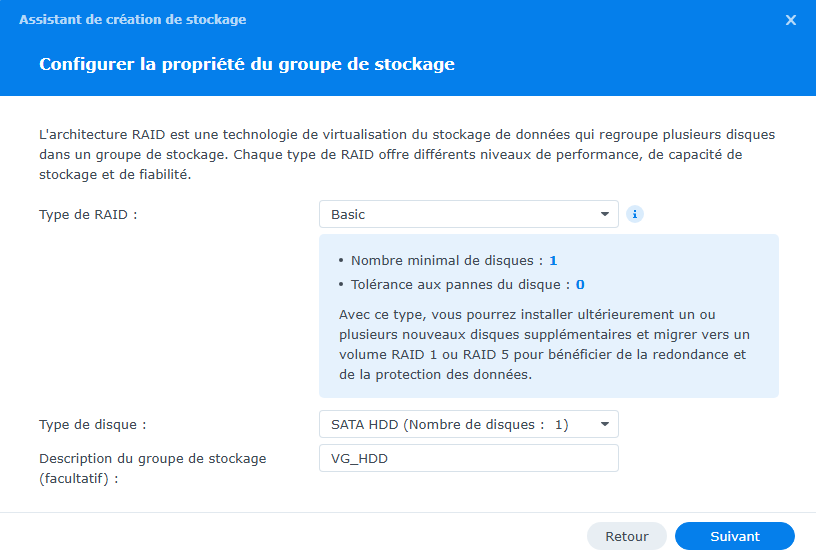
\includegraphics[width=0.9\textwidth]{03-Storage-config.tex/Images/03-storage-01.png}
    \caption{NAS - Stockage - Création d'un groupe de stockage}
    \label{fig:03-storage-01}
\end{figure}

\begin{figure}[H]
    \centering
    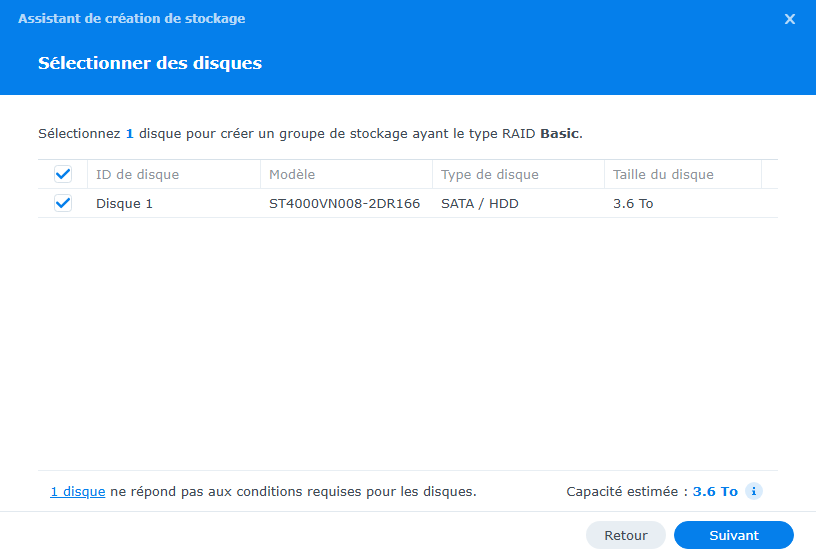
\includegraphics[width=0.9\textwidth]{03-Storage-config.tex/Images/03-storage-02.png}
    \caption{NAS - Stockage - Choix des disques}
    \label{fig:03-storage-02}
\end{figure}

\begin{figure}[H]
    \centering
    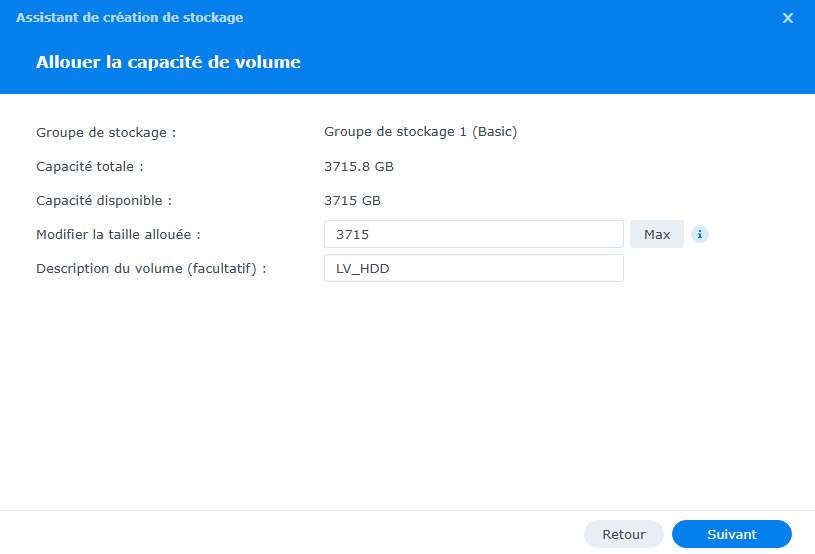
\includegraphics[width=0.9\textwidth]{03-Storage-config.tex/Images/03-storage-03.png}
    \caption{NAS - Stockage - Création du volume logique}
    \label{fig:03-storage-03}
\end{figure}

\begin{figure}[H]
    \centering
    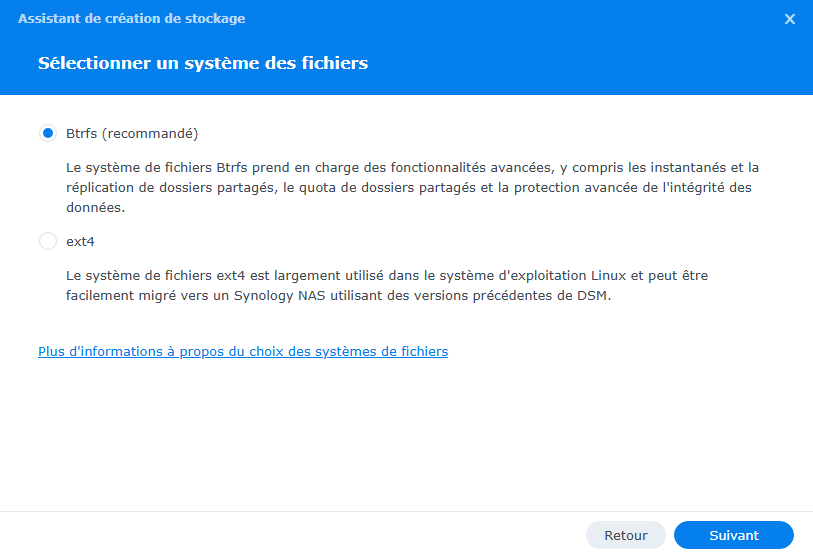
\includegraphics[width=0.9\textwidth]{03-Storage-config.tex/Images/03-storage-04.png}
    \caption{NAS - Stockage - Choix du système de fichiers}
    \label{fig:03-storage-04}
\end{figure}

Le volume logique est créé. Il est intéressant de planifier un nettoyage régulier des données.
\begin{itemize}
    \item Ouvrir le \textit{Gestionnaire de stockage}
    \item Accéder à la partie \textit{Stockage}
    \item Cliquer sur \textit{Planifier le nettoyage de données}
    \item Activer le nettoyage de données par défaut pour l'ensemble des groupes de stockage (figure \ref{fig:03-cleaner-01})
\end{itemize}

\begin{figure}[H]
    \centering
    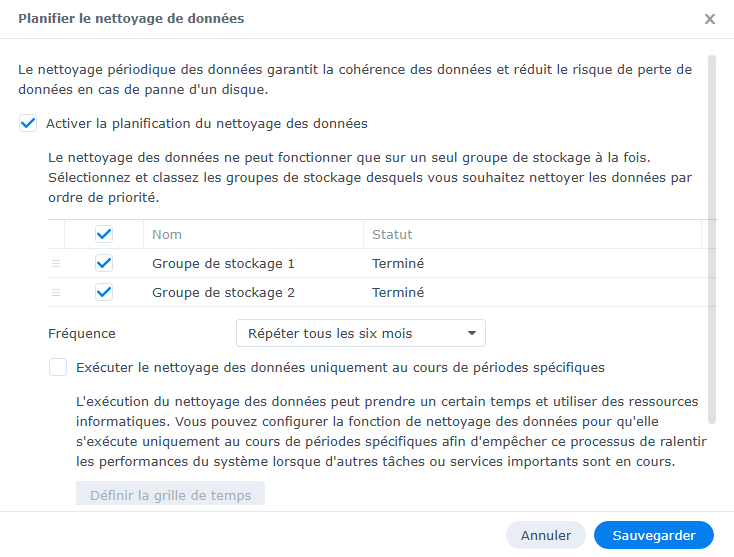
\includegraphics[width=0.9\textwidth]{03-Storage-config.tex/Images/03-cleaner-01.png}
    \caption{NAS - Stockage - Planification du nettoyage de données}
    \label{fig:03-cleaner-01}
\end{figure}